\section{Model 2}
As seen from the analysis above for the first model, the stationary solution for a circle of dense points would not approach the point set except for $\alpha=1$. Also, if the point set was not as dense, the curvature would be low near the points and conversely high far away.

The idea behind model 2 is to aim for the opposite, meaning a curve with high curvature near the points and approaching straight lines further away. This will be more similar to smoothed polygons with the sampled points as edges. 

In order to do so, the distance dependent function $f_2(d(\mathbf{x}; V)$ is chosen to be inversely proportional to the distance, and thus defined as
\begin{equation}
    f_2(d(\mathbf{x}; V) = \frac{\sigma(\mathbf{x}, t)}{\beta d(\mathbf{x})+\delta},
    \label{eq:f-2}
\end{equation}
Hence $f_2(d(\mathbf{x}; V)$ will be large close to the point set yielding a stationary solution of high curvature. Furthermore, the distance-dependent term in the energy function will be similar to a gravitational field, attracting more and more the closer to the source. The resulting model is obtained by inserting \eqref{eq:f-2} into \eqref{eq:general-model-pde}.

\begin{tcolorbox}[title=Model 2]
\begin{equation}
    u_t = |\nabla u| \bigg(\alpha \frac{ \sigma(\mathbf{x}, t)}{\beta d(\mathbf{x})+\delta} + (1-\alpha)\kappa (u) \bigg), \qquad \alpha, \beta, \delta \in \realspacem
    \label{eq:model2-pde}
\end{equation}
\end{tcolorbox}
Where the parameter $\delta>0$ avoids the velocity having a singularity at points in the point set and the term $\beta>0$ is a scaling parameter. Without varying the parameter $\beta$ with the domain size, identical point sets of different scalings will yield different curves.

\subsection{Radially Symmetric Analysis}
We conduct the same analysis for model 2 as for model 1. Using \eqref{eq:curvature-circle} and \eqref{eq:nablau-ur} and that $d(r)=|r-r_v|$, we obtain a radially dependent normal velocity
\begin{equation}
    v_n = \frac{\alpha \sigma(r_{\Gamma}, t)}{\beta (|r-r_v|)+\delta} + \frac{1-\alpha}{r}.
    \label{eq:general-inverse-velocityfield}
\end{equation}
Following the procedure for model 1 further, we find that the ODE for the characteristics/streamlines for the level curves is defined by $r_t = -v_n$ and using \eqref{eq:sigma-radius-1}-\eqref{eq:sigma-radius-2} to rewrite $\sigma(r, t)$ and inserting into \eqref{eq:general-inverse-velocityfield} we get the velocity for all level curves with a radius $r(t)$, as 
\begin{alignat}{3}
    r_t &= -&\bigg(\frac{\alpha }{\beta(|r(t)-r_v|)+\delta} + \frac{1-\alpha}{r(t)}\bigg) \qquad &\text{if }r_{\Gamma} \geq r_v,\\
    r_t &= &\bigg(\frac{\alpha}{\beta(|r(t)-r_v|)+\delta} -  \frac{1-\alpha}{r(t)}\bigg) \qquad &\text{if }r_{\Gamma} < r_v.
\end{alignat}

Because we add the small constant $\delta$ to the denominator in \eqref{eq:general-inverse-velocityfield} we cannot in the same manner as for \eqref{eq:pde-zero-streamline} remove the absolute value for the zero level curve because the sign of $\delta$ should also be changed when $r(t)=r_v$. For the zero level curve, we then get the set of equations which applies for the two cases when the curve is outside or inside the point set.
\begin{alignat}{3}
    r_t &= -&\bigg(\frac{\alpha}{\beta(r(t)-r_v)+\delta} + \frac{(1-\alpha)}{r(t)}\bigg) \quad &\text{for }r(t) = r_{\Gamma}>r_v, \label{eq:pde-zero-streamline-inverse-1} \\
    r_t &= &\bigg(\frac{\alpha}{\beta(r_v - r(t))+\delta} -  \frac{(1-\alpha)}{r(t)}\bigg) \quad &\text{for }r(t) = r_{\Gamma}>r_v.\label{eq:pde-zero-streamline-inverse-2}
\end{alignat}
    

Thus, solving \eqref{eq:pde-zero-streamline-inverse-1} and \eqref{eq:pde-zero-streamline-inverse-2} with $r_t=0$ gives the stationary solution, $r_f$. We begin with \eqref{eq:pde-zero-streamline-inverse-1} which yields  
\begin{equation*}
\begin{cases}
    r_f = \frac{\beta (1-\alpha)}{\alpha + \beta (1-\alpha)} (r_v-\delta/\beta), \\
    r_f > r_v.
\end{cases}
\end{equation*}
We see that for all choices of $\alpha \in [0, 1]$, $\delta>0$ and $\beta>0$, $r_f$ will have to be smaller than $r_v$. This does not satisfy the constraint $r_f>r_v$, and thus the stationary solution of \eqref{eq:pde-zero-streamline-inverse-1} is not feasible. We proceed to look at the situation where $r_{\Gamma}<r_v$ in \eqref{eq:pde-zero-streamline-inverse-2} which has the stationary solution
\begin{equation}
\begin{cases}
    r_f = \frac{\beta (1-\alpha)}{\alpha + \beta (1-\alpha)} (r_v+\delta/\beta), \\
    r_f < r_v.
\end{cases}
\label{eq:stationary-sol-inverse}
\end{equation}
Neither for \eqref{eq:stationary-sol-inverse}, the stationary radius is guaranteed to exist but depends in the parameter choices. Furthermore, we see that we can make $r_f \sim r_v$ by choosing $\delta$ small and $\alpha$ big, but we see in \figref{fig:total-streamline-inverse} that this solution is unstable. \todo{Vis at stasjonær løsning ustabil}

\begin{figure}
    \begin{subfigure}{.5\linewidth}
        \centering
        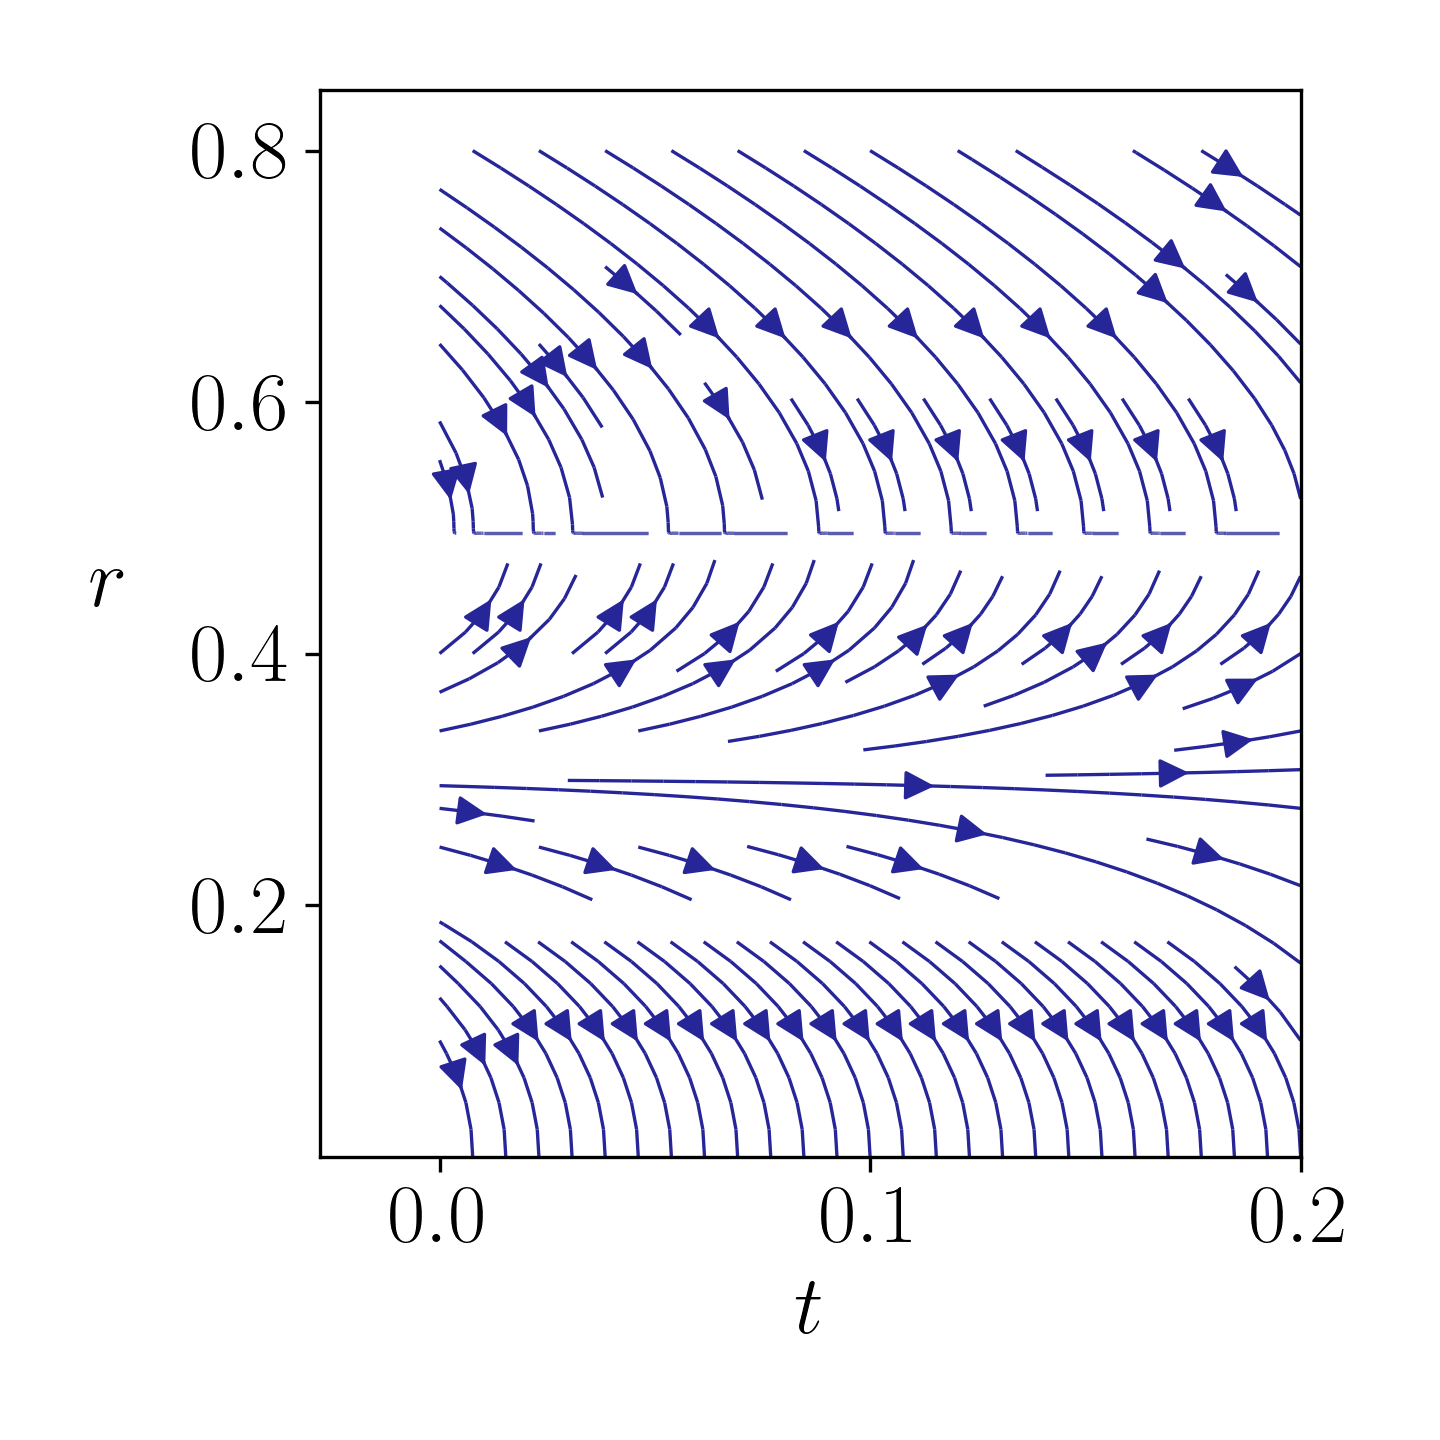
\includegraphics[width=\linewidth]{figures/streamlines/mod2-a40.png}
        \caption{$\alpha=0.4$}
        \label{fig:inverse-sub1}
    \end{subfigure}%
    \begin{subfigure}{.5\linewidth}
        \centering
        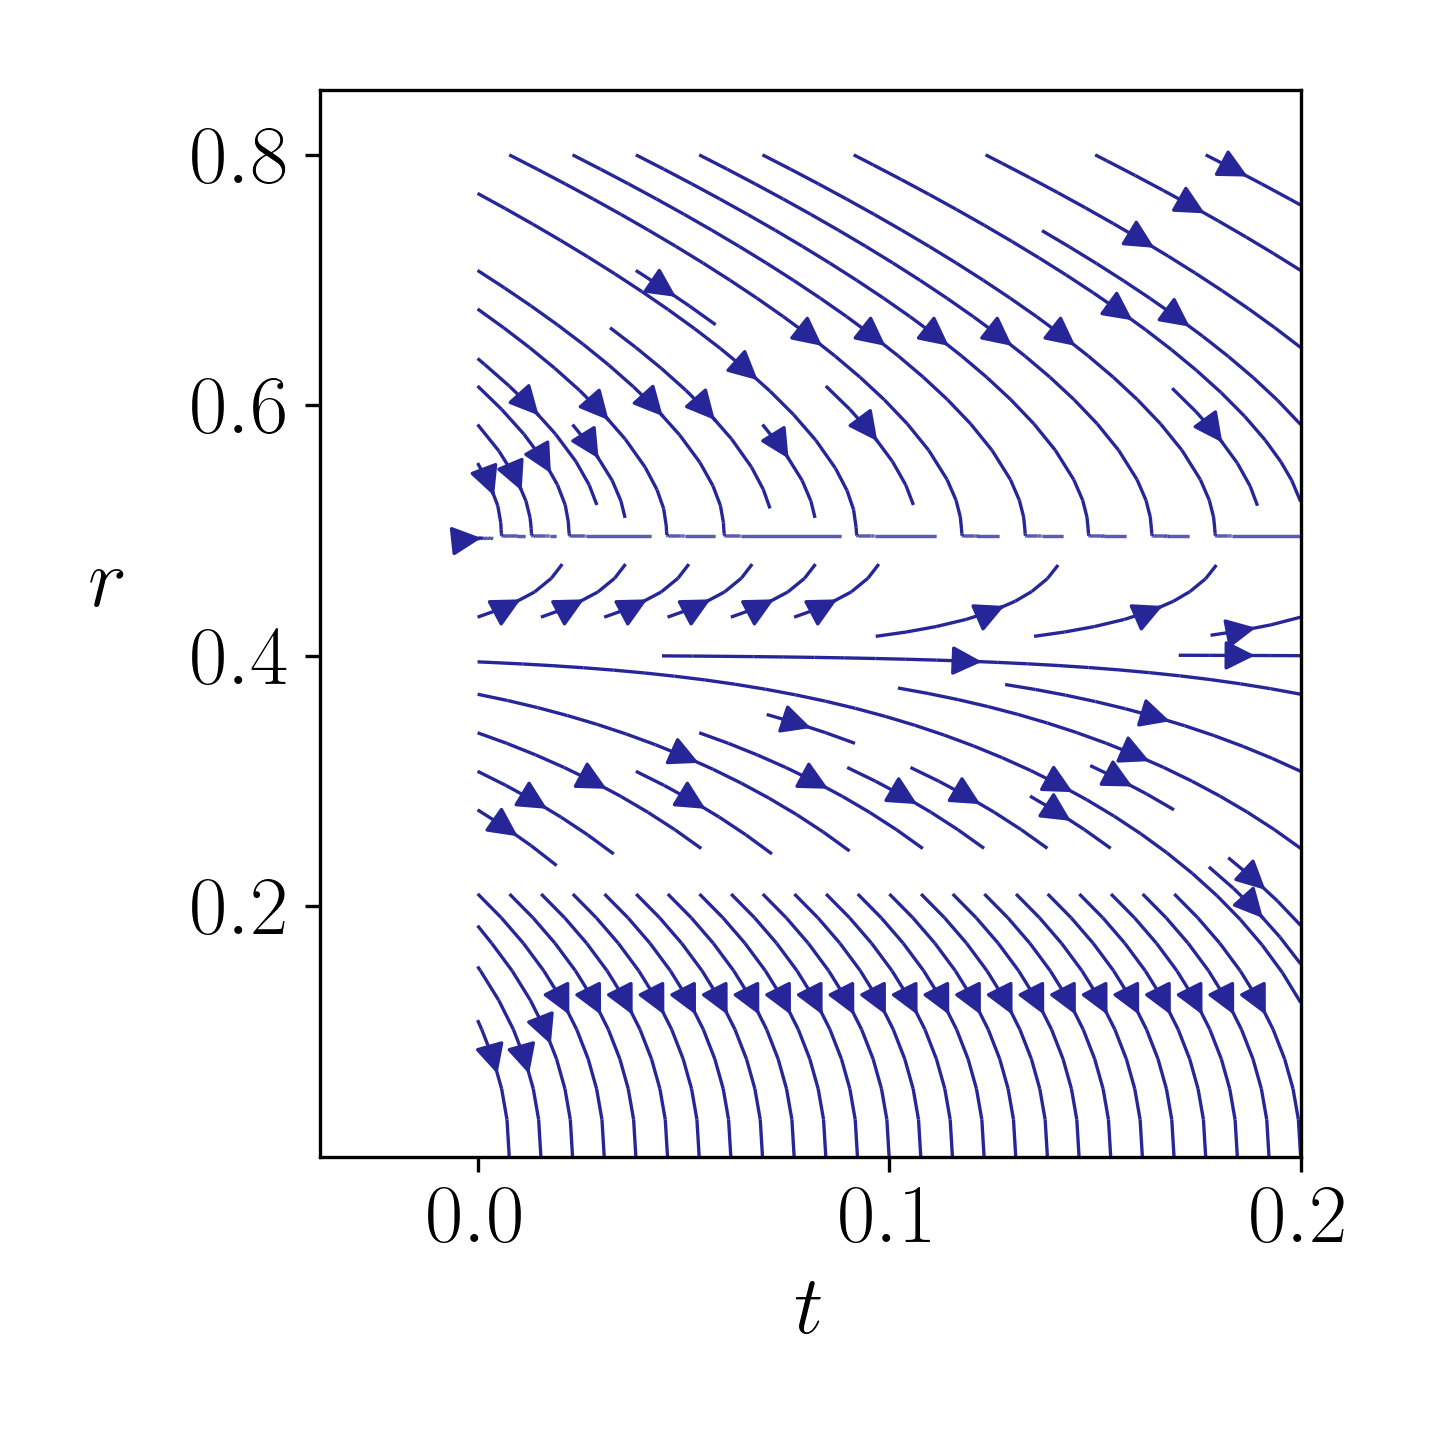
\includegraphics[width=\linewidth]{figures/streamlines/mod2-a20.png}
        \caption{$\alpha=0.2$}
        \label{fig:inverse-sub2}
    \end{subfigure}
    \caption[Streamlines for alternative velocity field]{Streamlines for the zero level set curve, $\Gamma(t)$, in the radially symmetric situation with the point set, \pointset, situated at $r_v=0.5$ and for the velocity field depending on the inverse distance \eqref{eq:general-inverse-velocityfield}.}
    \label{fig:total-streamline-inverse}
\end{figure}

Also, as we did above, we look at the streamlines for the zero level set curves starting at different initial radii in \figref{fig:total-streamline-inverse} for $\alpha=0.4$ and $\alpha=0.96$. Notice the difference in time scale from \figref{fig:total-streamline-picture} to \figref{fig:total-streamline-inverse}, where we see that the velocities are much grater when $r_{\Gamma}$ approaches $r_v$. It could also appear from \figref{fig:total-streamline-inverse} that we have a stable solution in $r_{\Gamma}=r_v$, but when inserting this into the equations for the curve velocity $r_v$ in \eqref{eq:pde-zero-streamline-inverse-1} and \eqref{eq:pde-zero-streamline-inverse-2}, we get

\begin{alignat}{3}
    r_t &= -&\bigg(\frac{\alpha}{\delta} + \frac{(1-\alpha)}{r_v}\bigg) \quad &\text{for }r(t) = r_{\Gamma}\geq r_v, \label{eq:pde-streamline-inverse-1}\\
    r_t &= &\bigg(\frac{\alpha}{\delta} -  \frac{(1-\alpha)}{r_v}\bigg) \quad &\text{for }r(t) = r_{\Gamma}<r_v,\label{eq:pde-streamline-inverse-2}
\end{alignat}
which is non-zero for $\delta \neq (\alpha r_v)/(1-\alpha)$. We thus have observed a discontinuity in the velocity function at $r=r_v$, where the velocity is very high in opposite directions slightly inwards or outwards of the point set radius, $r_v$. This will mean that if we solve this equation numerically, we will observe oscillations around the radius of the point set.

This oscillating behavior is very important to notice, because as we now have seen, there is no guarantee that we will obtain a stationary solution for all configurations of point sets. In order to obtain a stationary solution, a specific relation between curvature and distance must be fulfilled, and we see now that if the points are too densely spaced, there is not enough space to obtain the high curvature needed to balance the distance function.

In fact solving \eqref{eq:model2-pde} with $u_t=0$ for the curvature, yields a distance-curvature relation where the sign is decided by $\sigma$ locally: 
\begin{equation}
    \kappa (u) = \pm \frac{\alpha}{(1-\alpha)(\beta \distanceVm+\delta)}.
    \label{eq:dist-curv-relation-m2}
\end{equation}
From this, we see that in order to satisfy this, the curvature will be high close to the points and further and further away from the points, the curvature will decrease and yield straighter and straighter curves.

Further more, we can for model 2 not make a similar streamline picture as \figref{fig:total-streamline-picture} where we view the streamlines for all level curves given an initial radius for the zero level curve. For model 1, we got that the sign only changed once and the time of the sign change could be calculated, but for model 2, the sign will change infinitely fast and infinitely many times. 

We thus do not get as much information about model 2 for this radially symmetric situation. But this is an interesting result as well, because we have seen that not all point sets for all models yield a stationary solution at all. We have here seen that the zero level curve will stop at the point set for the provided example, but the requirement that $r_t=0$ is not fulfilled.

\begin{comment}
\textit{What do I have to say in this section?}
\begin{enumerate}
    \item Curve stationary (oscillating) when covering the point set
    \item Straight lines between, high curvature close
    \item Oscillation, and high velocities close to points
    \item $\kappa(u)=-\frac{\alpha}{1-\alpha} 1/(d+\delta)$.
\end{enumerate}
\end{comment}
